\section{Auswertung}
\subsection{Kennlinie der Pumpe} \label{sec:230514_Kennlinie_der_Pumpe}
Damit die Pumpenkennlinie dargestellt werden kann, müssen die gemessenen Ströme für den Volumenstrom und den Druck erst in verwwendbare Einheiten umgewandelt werden. 
Hierzu werden Proportionalitätsfaktoren und Kalibrieungsoffsets benötigt. 
Die Offsets wurden gemessen und batragen $I_{off,Q}=4,05 mA$ und $I_{off,p}=5,868 mA$.
Die Proportionalitätsfaktoren wurden in der Versuchsanleitung gegeben und betragen $K_Q = 6,3 \frac{l}{min \cdot mA}$ und $K_p = 0,6 \frac{bar}{mA}$.
Die Volumenströme in $\frac{m^3}{h}$ lassen sich mittels \autoref{eq:230513_Volumenstrom} berechnen und die Drücke in bar mittels \autoref{eq:230513_Druck}.
\begin{equation}
  Q = (I_{mess}-I_{off,Q})\cdot K_Q \cdot \frac{60\frac{min}{h}}{1000\frac{l}{m^3}}
  \label{eq:230513_Volumenstrom}
\end{equation}

\begin{equation}
  p = (I_{mess}-I_{off,p})\cdot K_p
  \label{eq:230513_Druck}
\end{equation}

Des wieteren müssen die Drücke in Förderhöhen umgewandelt werden. Hierzu wird die gravitationknostante $g = 9,81 \frac{m}{s^2}$ und die Dichte des Wassers $\rho = 998 \frac{kg}{m^3}$ benötigt.
Dies erfolgt mit \autoref{eq:230513_Förderhöhe}, wobei der Druck in Pascal und nicht in bar angegeben werden muss.

\begin{equation}
  H = \frac{p}{\rho \cdot g}
  \label{eq:230513_Förderhöhe}
\end{equation}

Aus den im Anhang gegebenen Messtabelln ergibt sich die \autoref{fig:230513_Pumpenkennlinie}.
\begin{figure}[!ht]
  \centering
  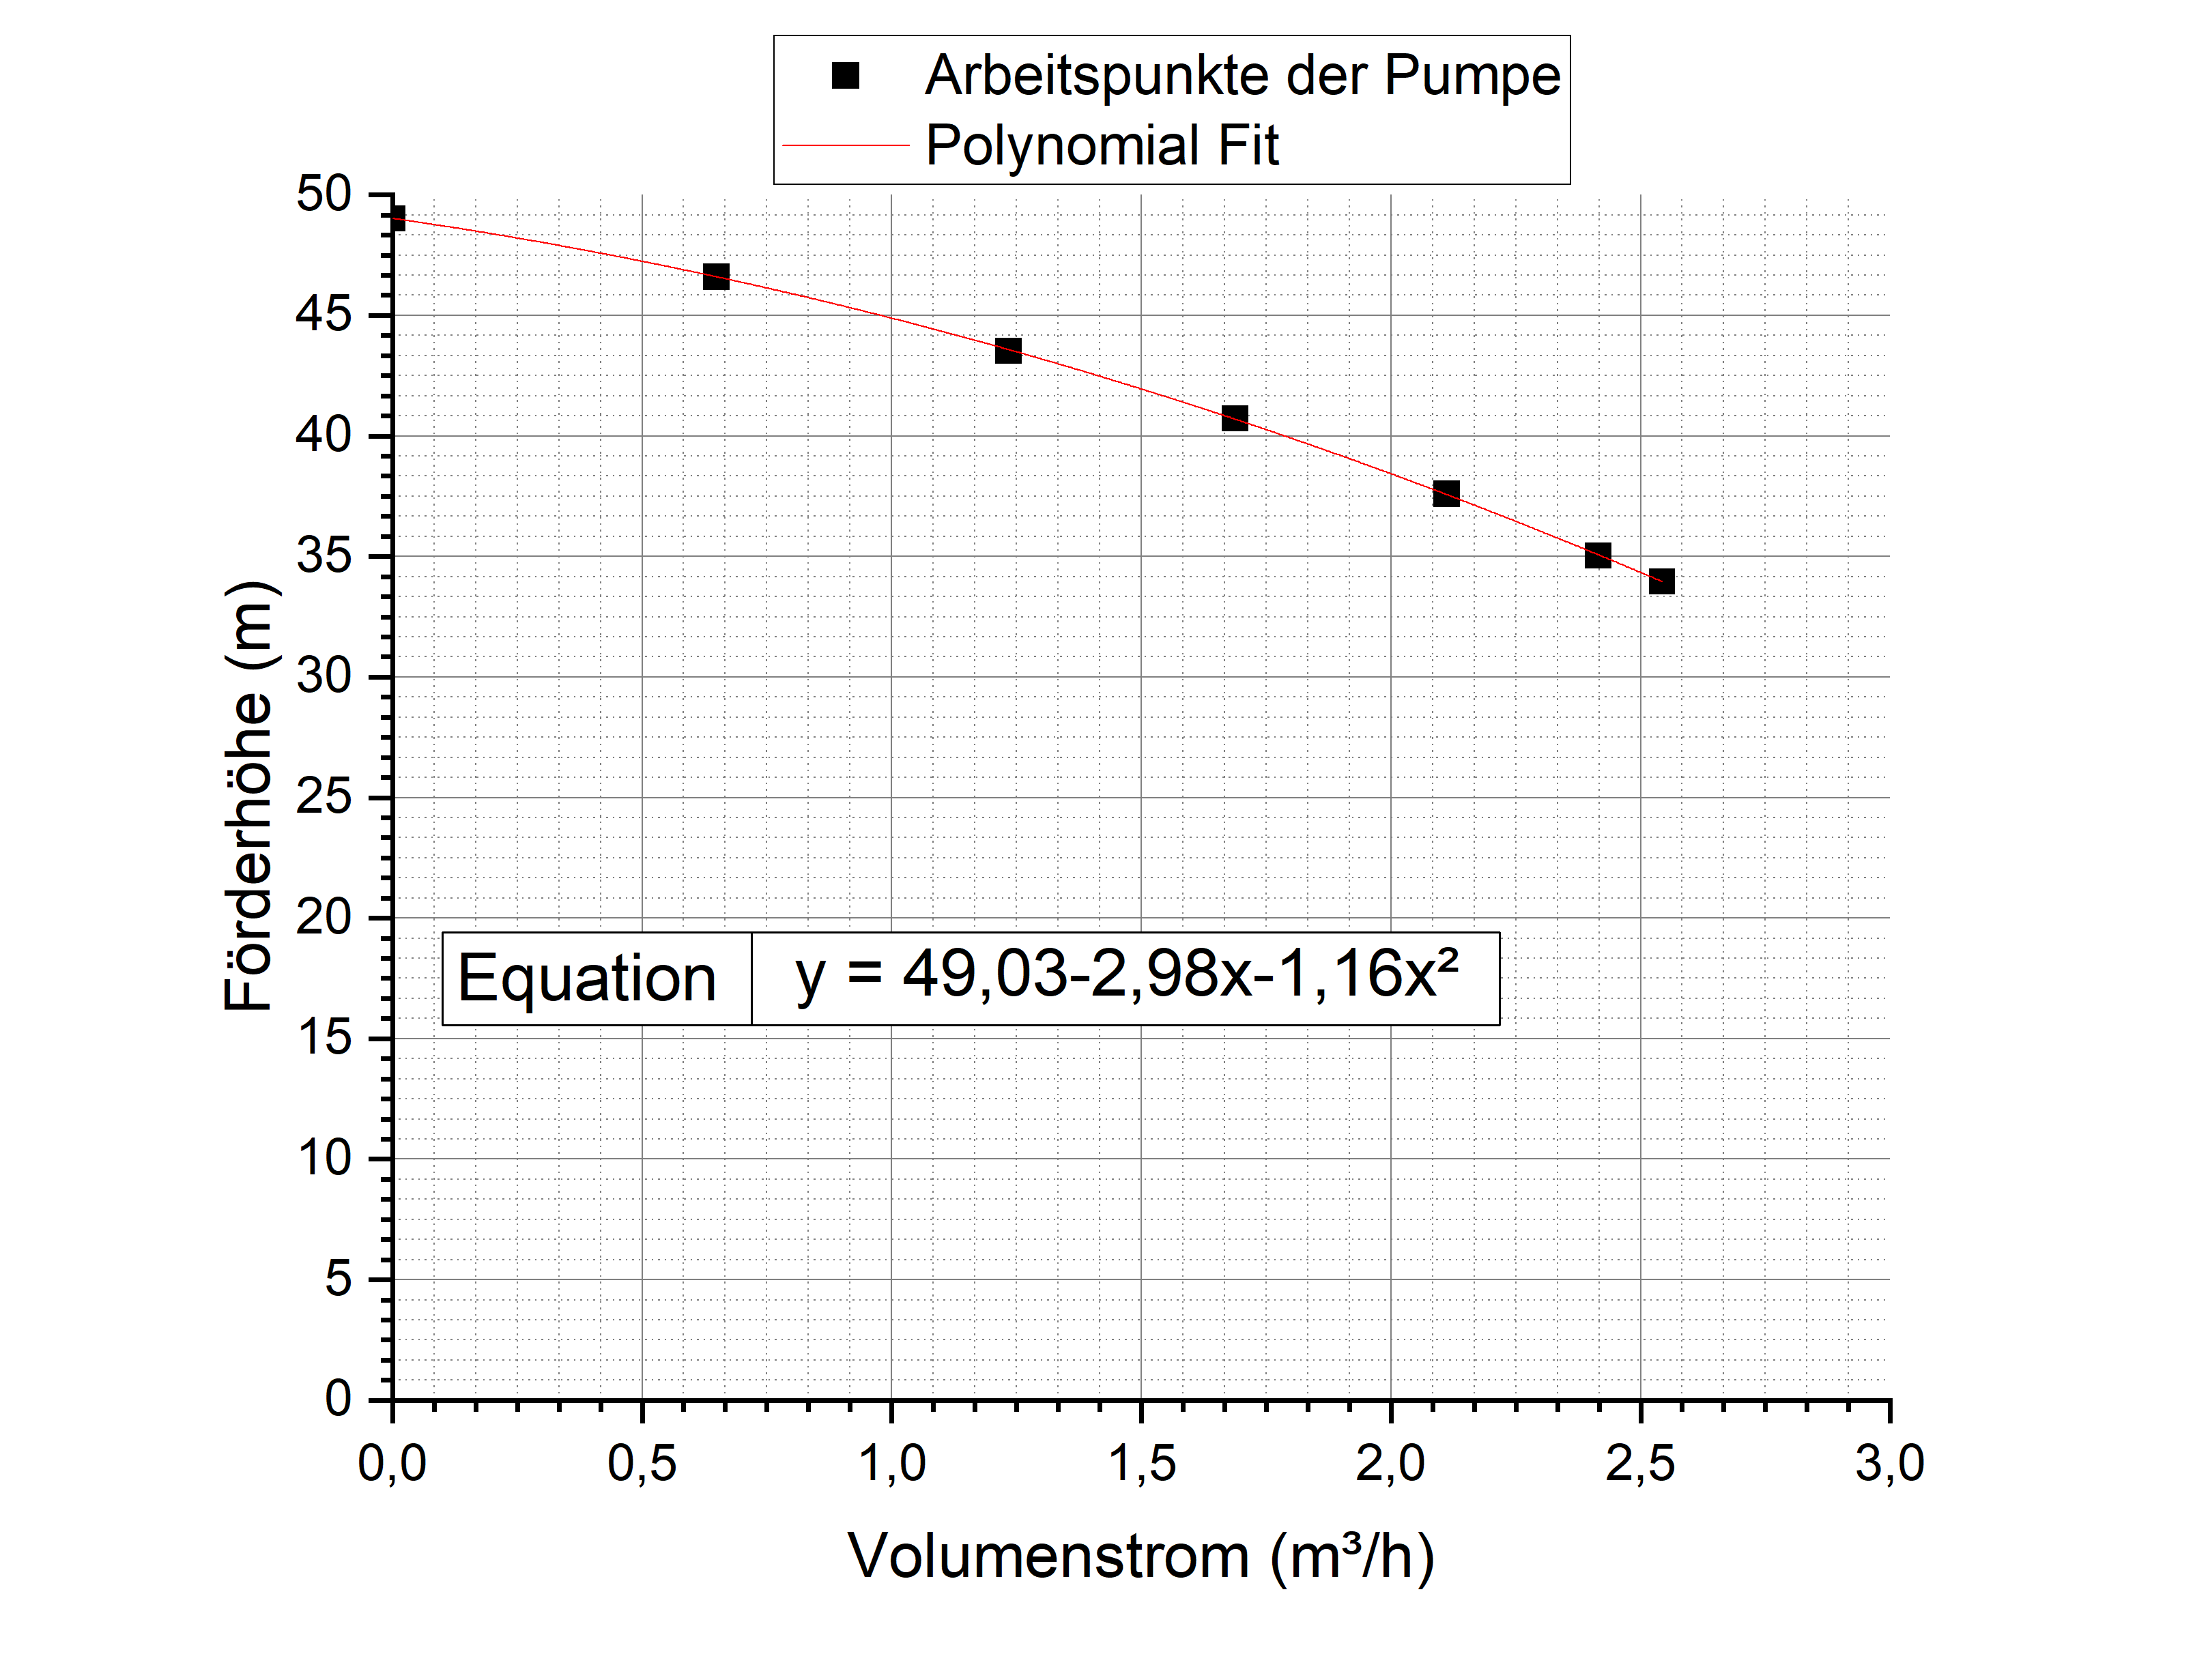
\includegraphics[width=0.8\textwidth]{Abbildungen/Pumpenkennlinie.png}
  \caption{Pumpenkennlinie bei gemessenen Arbeitspunkten}
  \label{fig:230513_Pumpenkennlinie}
\end{figure}

\subsection{Betriebspunkte der Pelton-Turbine}
\subsubsection{Berechnen Sie die hydraulische Leistung, die mechanische Leistung und die elektrische Leistung in jedem Arbeitspunkt.}
Zur berechnung der hydraulischen Leistung werden erneut die Volumenströme und Förderhöhen benötigt, welche Analog zu dem vorgehen in \autoref{sec:230514_Kennlinie_der_Pumpe} berechnet wurden.
Die hydraulische Leistung wird mittels \autoref{eq:230514_hydraulische_Leistung} berechnt:

\begin{equation}
  P_{Hyd.} = \rho \cdot g \cdot Q \cdot H
  \label{eq:230514_hydraulische_Leistung}
\end{equation}

Die mechanische Leistung lässt sich mittels \autoref{eq:230514_mechanische_Leistung} berechnen.
Jedoch mussten zuerst die Messwerte des Kraftsensors ausgewertet und in ein Moment umgerechnet werden.
Dieser hat zeitreihen der ausgeübten Kraft aufgezeichnet, von welchen die Mittelwerte gebildet wurden.
Anschließend wurden diese Kräft mit der Länge des Hebelarms $l = 290 mm$ verrechnet, um ein Moment heraus zu bekommen.

\begin{equation}
  P_{Mech.} = M \cdot 2 \pi \cdot n
  \label{eq:230514_mechanische_Leistung}
\end{equation}

Die elektrische Leistung lies sich durch die Gemessenen Phasenströme und -Spannungen mittels \autoref{eq:230514_elektrische_Leistung} berechen:

\begin{equation}
  P_{El.} = U \cdot I
  \label{eq:230514_elektrische_Leistung}
\end{equation}

Die Leistungen bei den verschiedenen Arbeitspunkten lassen sich in \autoref{tab:230514_Arbeitspunkte} finden.
\begin{table}[!ht]
  \caption{Drehzahlen,Leistungen und Wirkungsgrade der Pelton Turbine bei verschiedenen Arbeitspunkten}
  \centering
  \begin{tabular}{|l|l|l|l|l|}
      \hline
      \rowcolor[HTML]{70AD47} 
      Drehzahl in $min^-1$ & $P_{hyd.}$ in $W$ & $P_{Mech.}$ in $W$ & $P_{El.}$ in $W$ & \cellcolor[HTML]{5B9BD5}$\eta_{Turbine}$ \\ \hline \hline
      \rowcolor[HTML]{E2EFDA} 
      \rowcolor[HTML]{E2EFDA} 
      3180                                & 298,927      & -2,014        & 0,533       & \cellcolor[HTML]{DDEBF7}-0,67\%      \\ \hline
      \rowcolor[HTML]{A9D08E} 
      3130                                & 297,214      & 1,325         & 42,990      & \cellcolor[HTML]{BDD7EE}0,45\%       \\ \hline
      \rowcolor[HTML]{E2EFDA} 
      2970                                & 296,785      & 23,337        & 142,288     & \cellcolor[HTML]{DDEBF7}7,86\%       \\ \hline
      \rowcolor[HTML]{A9D08E} 
      2800                                & 296,785      & 40,993        & 258,249     & \cellcolor[HTML]{BDD7EE}13,81\%      \\ \hline
      \rowcolor[HTML]{E2EFDA} 
      2600                                & 296,785      & 50,566        & 363,731     & \cellcolor[HTML]{DDEBF7}17,04\%      \\ \hline
      \rowcolor[HTML]{A9D08E} 
      2430                                & 296,357      & 59,603        & 438,209     & \cellcolor[HTML]{BDD7EE}20,11\%      \\ \hline
      \rowcolor[HTML]{E2EFDA} 
      2230                                & 295,929      & 60,693        & 473,889     & \cellcolor[HTML]{DDEBF7}20,51\%      \\ \hline
      \rowcolor[HTML]{A9D08E} 
      2050                                & 295,029      & 62,358        & 482,203     & \cellcolor[HTML]{BDD7EE}21,14\%      \\ \hline
      \rowcolor[HTML]{E2EFDA} 
      1930                                & 294,579      & 58,116        & 482,203     & \cellcolor[HTML]{DDEBF7}19,73\%      \\ \hline
      \rowcolor[HTML]{A9D08E} 
      1820                                & 294,130      & 57,654        & 473,889     & \cellcolor[HTML]{BDD7EE}19,60\%      \\ \hline
      \rowcolor[HTML]{E2EFDA} 
      1750                                & 294,130      & 57,198        & 473,889     & \cellcolor[HTML]{DDEBF7}19,45\%      \\ \hline
      \rowcolor[HTML]{A9D08E} 
      1640                                & 292,830      & 53,868        & 491,036     & \cellcolor[HTML]{BDD7EE}18,40\%      \\ \hline
      \rowcolor[HTML]{E2EFDA} 
      1360                                & 292,830      & 51,171        & 461,418     & \cellcolor[HTML]{DDEBF7}17,47\%      \\ \hline
      \rowcolor[HTML]{A9D08E} 
      1220                                & 293,727      & 46,710        & 423,573     & \cellcolor[HTML]{BDD7EE}15,90\%      \\ \hline
      \rowcolor[HTML]{E2EFDA} 
      1100                                & 293,727      & 43,527        & 389,711     & \cellcolor[HTML]{DDEBF7}14,82\%      \\ \hline
      \rowcolor[HTML]{A9D08E} 
      970                                 & 292,427      & 38,550        & 346,757     & \cellcolor[HTML]{BDD7EE}13,18\%      \\ \hline
      \rowcolor[HTML]{E2EFDA} 
      875                                 & 292,852      & 35,740        & 321,555     & \cellcolor[HTML]{DDEBF7}12,20\%      \\ \hline
      \rowcolor[HTML]{A9D08E} 
      795                                 & 292,427      & 33,160        & 305,361     & \cellcolor[HTML]{BDD7EE}11,34\%      \\ \hline
      \rowcolor[HTML]{E2EFDA} 
      705                                 & 292,405      & 30,200        & 276,435     & \cellcolor[HTML]{DDEBF7}10,33\%      \\ \hline
      \rowcolor[HTML]{A9D08E} 
      610                                 & 292,874      & 26,396        & 241,101     & \cellcolor[HTML]{BDD7EE}9,01\%       \\ \hline
      \rowcolor[HTML]{E2EFDA} 
      535                                 & 292,427      & 23,772        & 218,238     & \cellcolor[HTML]{DDEBF7}8,13\%       \\ \hline
  \end{tabular}
  \label{tab:230514_Arbeitspunkte}
\end{table}

\subsubsection{Bestimmen Sie den Turbinenwirkungsgrad und tragen diesen grafisch über der Drehzahl auf.}
Die Turbinen Wirkungsgrade können durch \autoref{eq:230512_Turbinenwirkungsgrad} berechnet und werden in \autoref{tab:230514_Arbeitspunkte} Numerisch und in \autoref{fig:230514_Wirkungsgrade} grafisch über die Drehzahl abgebildet. 

\begin{equation}
  \eta_{Turbine} = \frac{P_{Hyd.}}{P_{Mech.}}
  \label{eq:230512_Turbinenwirkungsgrad}
\end{equation}

\begin{figure}[H]
  \centering
  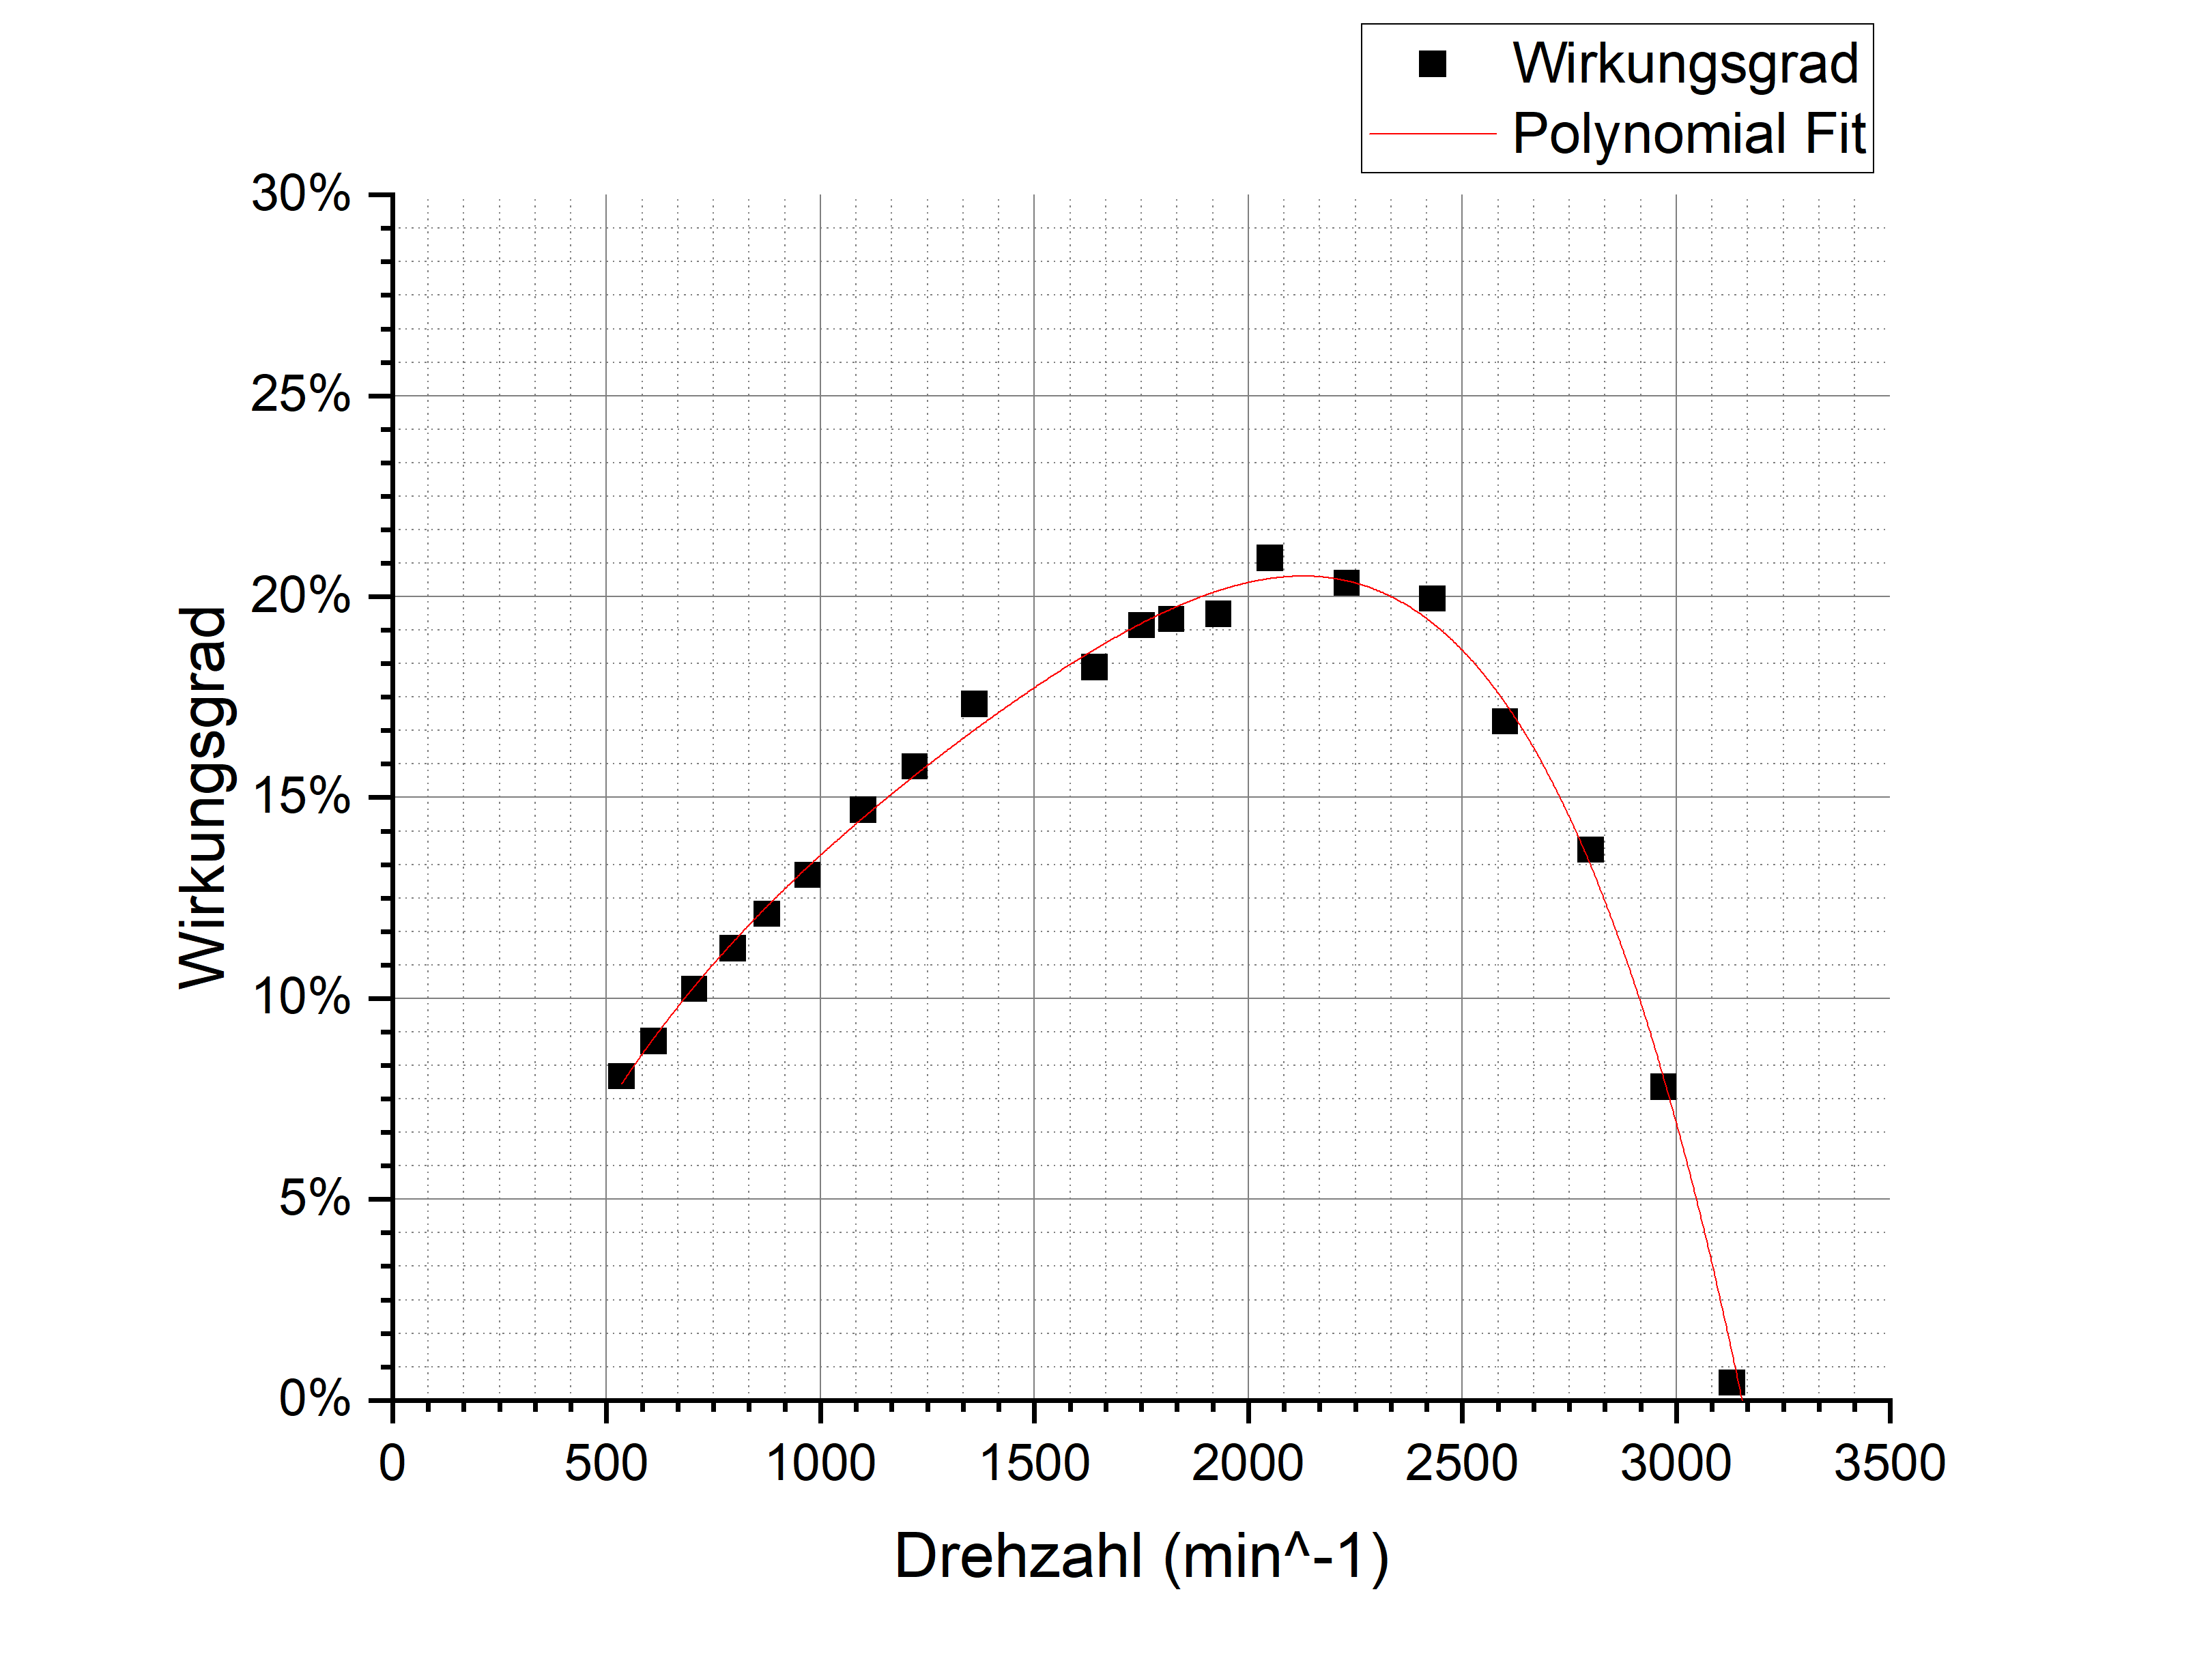
\includegraphics[width=0.9\textwidth]{Abbildungen/Wirkungsgrade.png}
  \caption{Turbinenwirkungsgrade über die Drehzahl}
  \label{fig:230514_Wirkungsgrade}
\end{figure}

\subsubsection{Vergleichen Sie den Arbeitspunkt mit bestem Wirkungsgrad mit den theoretischen Betrachtungen}
\subsubsection{Interpretieren Sie evtl. auftretende Abweichungen des optimalen Arbeitspunkts.}

\subsection{Verlustbeiwert der Düse}